%--------------------
% Packages
% -------------------
\documentclass[11pt,a4paper]{article}
\usepackage[utf8x]{inputenc}
\usepackage[T1]{fontenc}
\usepackage{booktabs} % For nice tables
\usepackage{siunitx}
\usepackage[pdftex]{graphicx} % Required for including pictures
\usepackage[pdftex,linkcolor=black,pdfborder={0 0 0}]{hyperref} % Format links for pdf
\usepackage{calc} % To reset the counter in the document after title page
\usepackage{enumitem} % Includes lists
\usepackage[a4paper, lmargin=1in, rmargin=1in, tmargin=1in, bmargin=1in]{geometry} %margins
\usepackage{fancyhdr}
\usepackage[all]{nowidow} % Tries to remove widows
\usepackage[protrusion=true,expansion=true]{microtype} % Improves typography, load after fontpackage is selected
\usepackage{lipsum} % Used for inserting dummy 'Lorem ipsum' text into the template
\usepackage{listings,newtxtt}
\usepackage{xcolor}
\usepackage{titling}
\usepackage{blindtext}
\usepackage{tabularx}

\bibliographystyle{unsrt}

\definecolor{codegreen}{rgb}{0,0.6,0}
\definecolor{codegray}{rgb}{0.5,0.5,0.5}
\definecolor{codepurple}{rgb}{0.58,0,0.82}
\definecolor{backcolour}{rgb}{0.95,0.95,0.92}

\lstdefinestyle{mystyle}{
  backgroundcolor=\color{backcolour},
  commentstyle=\color{codegreen},
  keywordstyle=\color{magenta},
  numberstyle=\tiny\color{codegray},
  stringstyle=\color{codepurple},
  basicstyle=\ttfamily\footnotesize,
  breakatwhitespace=false,
  breaklines=true,
  captionpos=b,
  keepspaces=true,
  showspaces=false,
  showstringspaces=false,
  showtabs=false,
  tabsize=2,
  framexleftmargin=0pt,
  framexrightmargin=0pt,
  framextopmargin=6pt,
  framexbottommargin=6pt,
  frame=tb, framerule=0pt,
}

\lstset{style=mystyle}

%-----------------------
% Set pdf information and add title, fill in the fields
%-----------------------
\hypersetup{
pdfsubject = {},
pdftitle = {},
pdfauthor = {}
}

%-----------------------
% Begin document
%-----------------------

\fancypagestyle{firstpage}
{
\fancyhf{}
\renewcommand{\headrulewidth}{0pt} % removes horizontal header line
}

\pagestyle{fancy}

\fancyhf{}
\fancyhead[R]{\thepage}
\fancyhead[L]{Targeted Adversarial Examples for Air Traffic Speech Recognition}

\begin{document}

\title{Targeted Adversarial Examples for Air Traffic Speech Recognition}

\author{
  Andrew Dassonville\\
  \texttt{dassonva@oregonstate.edu}
  \and
  Austin Friedrich\\
  \texttt{friedrau@oregonstate.edu}
  \and
  Matthew Brayton\\
  \texttt{braytonm@oregonstate.edu}
}

\maketitle

\thispagestyle{firstpage}

\begin{abstract}
  We present a novel technique designed specifically for generating targeted
  adversarial examples aimed at compromising air traffic speech recognition
  systems. This method is leveraged to create adversarial pilot weather reports,
  also known as PIREPs, to target a speech recognition system that has been
  trained on an Air Traffic Control (ATC) dataset. We quantify the efficacy of
  our adversarial examples by computing the Character Error Rate (CER) of the
  speech recognition system, following the insertion of varying noise levels
  into these adversarial examples. Our results demonstrate that the method we
  propose can effectively generate adversarial examples that remain robust
  against realistic levels of noise typically encountered within radio
  communication channels.
\end{abstract}

\section{Introduction}

Since 2005, the Federal Aviation Administation (FAA) has been developing new
systems through its NextGen program to modernize the National Airspace System
(NAS), improving both safety and efficiency \cite{web:faa_nextgen}. As part of
this program, the FAA, in collaboration with NASA, has been investigating the
use of speech recognition systems to streamline various air traffic control
processes \cite{nasa-2016-speech-recognition}, and hope to begin deploying these
systems by 2024 \cite{faa-2022-nextgen}. Further, in 2022, Congress awarded the
FAA \$5 million to develop "advanced" safety methods, including machine learning
and speech recognition systems \cite{faa-2022-budget}.

One likely use of speech recognition systems in the NAS is to automate the entry
of pilot weather reports (PIREPs) into the weather databases
\cite{carstens2022accuracy}. Currently, air traffic controllers must manually
enter these reports, which can be time consuming and error prone, especially
during busy periods. Automating this process would allow controllers to focus on
other tasks, and would also allow for more accurate and timely weather reports.
Previous work \cite{carstens2022accuracy} has shown that although existing
commercial speech recognition systems are not yet accurate enough to be used for
this purpose, they are improving rapidly, and will likely be deployable in the
near future.

\subsection{Threat Model}

Although the benefits of speech recognition systems in the NAS are clear, the
introduction of machine learning systems into the NAS also introduces new
attack surface for malicious actors. In this paper, we propose a method for
generating targeted adversarial PIREPs for air traffic speech recognition
systems. These adversarial examples are designed to sound like short bursts of
radio static to a human listener, a relatively common occurrence in aircraft
communications. As such, these examples would be unlikely to raise suspicion
from on-frequency listeners, such as pilots or air traffic controllers.

For the purposes of this paper, we assume that the attacker has access to the
target speech recognition model (i.e. a white box attack). Although this is a
strong assumption, it is a reasonable upper-bound and worth considering due to
the safety-critical nature of aviation. It is also assumed that the attacker has
a method for transmitting the adversarial examples to the target speech model,
such as a hand-held aviation radio, which would be relatively easy for a bad
actor to obtain.

\section{Background}

In this section, we briefly review relevant background material for this paper.
We begin by discussing the Wav2Vec 2.0 model, which is the speech recognition
model used for our experiments. We then discuss the Character Error Rate (CER)
metric, which is used to quantify the efficacy of our adversarial examples.

\subsection{Wav2Vec Model}

For our experiments, we make use of the Wav2Vec 2.0 \cite{baevski2020wav2vec}
model. Wav2Vec 2.0 is a speech recognition model introduced by Facebook in 2020
that uses a self-supervised pre-training task to learn speech representations
from largely unlabeled data. The underlying architecture of Wav2Vec 2.0 consists
of two key components: a convolutional feature encoder and a transformer-based
context network.

\subsection{Character Error Rate}

The Character Error Rate (CER) is a frequently-used metric in speech
recognition. It is calculated as the Levenshtein distance (the minimum number of
single-character edits\textemdash insertions, deletions, or
substitutions\textemdash needed to change one word into the other) between the
predicted and target text, normalized by the length of the target text.

We define the Levenshtein distance as the following equation, where $a$ and $b$
are two strings, $|a|$ is the length of $a$, and $a[i]$ is the $i$th character of
$a$, and $tail(a)$ is the string $a$ with the first character removed.

\begin{equation}
  lev(a, b) = \left\{ \begin{array}{ll}
    |a| & \text{if } |b|=0, \\
    |b| & \text{if } |a|=0, \\
    lev(tail(a), tail(b)) & a[0] = b[0]\\
    1 + \min \left\{ \begin{array}{l}
        lev(tail(a), b) \\
        lev(a, tail(b)) \\
        lev(tail(a), tail(b))
      \end{array} \right. & \text{otherwise}
    \end{array} \right.
\end{equation}

Then the Character Error Rate is defined by the following equation, where $y$ is
the target text and $\hat{y}$ is the predicted text.

\begin{equation}
  \text{CER}(y, \hat{y}) = \frac{lev(y, \hat{y})}{|y|}
\end{equation}

\section{Proposed Method}
\label{sec:method}

Our method for generating adversarial PIREPs is based on the Projected Gradient
Descent (PGD) attack \cite{madry2017towards}. We begin by sampling 10 seconds of
noise from a Gaussian distribution with mean $\mu = 0$ and standard deviation
$\sigma = 0.1$.

\begin{equation}
  x_0 \sim \mathcal{N}(\mu, \sigma^2)
  \label{eq:noise}
\end{equation}

We use the Connectionist Temporal Classification (CTC)
\cite{graves2006connectionist} loss equation, which is commonly used for speech
recognition tasks, to calculate the loss between the target transcript and the
transcript generated by the speech recognition model.

\begin{equation}
  \mathcal{L}(y, \hat{y}) = - \log P_{CTC}(y | \hat{y})
\end{equation}

\begin{equation}
  P_{CTC}(y | \hat{y}) = \sum_{a \in \mathcal{B}^{-1}(y)} \prod_{t} P(a_t | \hat{y}_t)
\end{equation}

Using the loss equation, we use the following equation to take a step of PGD,
where $\alpha$ is the step size, $\epsilon$ is the attack bound, $x_t$ is the
current adversarial example, and $f_\theta$ is the pretrained Wav2Vec 2.0 model.

\begin{equation}
  x_{t+1} = \text{Clip}_{\epsilon} \Big( x_t + \alpha \cdot \text{sign} \left( \nabla_{x} \mathcal{L}(f_\theta(x_t), y) \right) \Big)
\end{equation}

\section{Experiments}

To evaluate the effectiveness of our method, we generate an adversarial PIREP
of a ficticious airplane reporiting the temperature, cloud bases, and light rime
icing conditions to Seattle Center. The target transcript is:

\begin{lstlisting}[breaklines]
  SEATTLE CENTER SKYHAWK TWO THREE ZULU PIREP TEMPERATURE MINUS FOUR CLOUD BASES THREE THOUSAND LIGHT RIME ICE ACCUMULATION
\end{lstlisting}

Using this transcript, we generate an adversarial PIREP with our method as
outlined in \autoref{sec:method}. We find that our method is able to quickly
generate targeted adversarial examples. With 300 iterations of PGD, we are able
to generate adversarial PIREPs with low CTC loss and a CER of less than 0.01.
This process takes less than 70 seconds on a single NVIDIA RTX A2000 GPU.

\autoref{fig:attack_loss_iteration} shows the CTC loss over 300 iterations of
PGD. Early iterations exhibit large spikes in CTC loss, but the loss quickly
converges to a low value. \autoref{fig:attack_cer_iteration} shows the CER over
300 iterations of PGD, which unsurprisingly follows a similar curve to the CTC
loss.

\begin{figure}
  \centering
  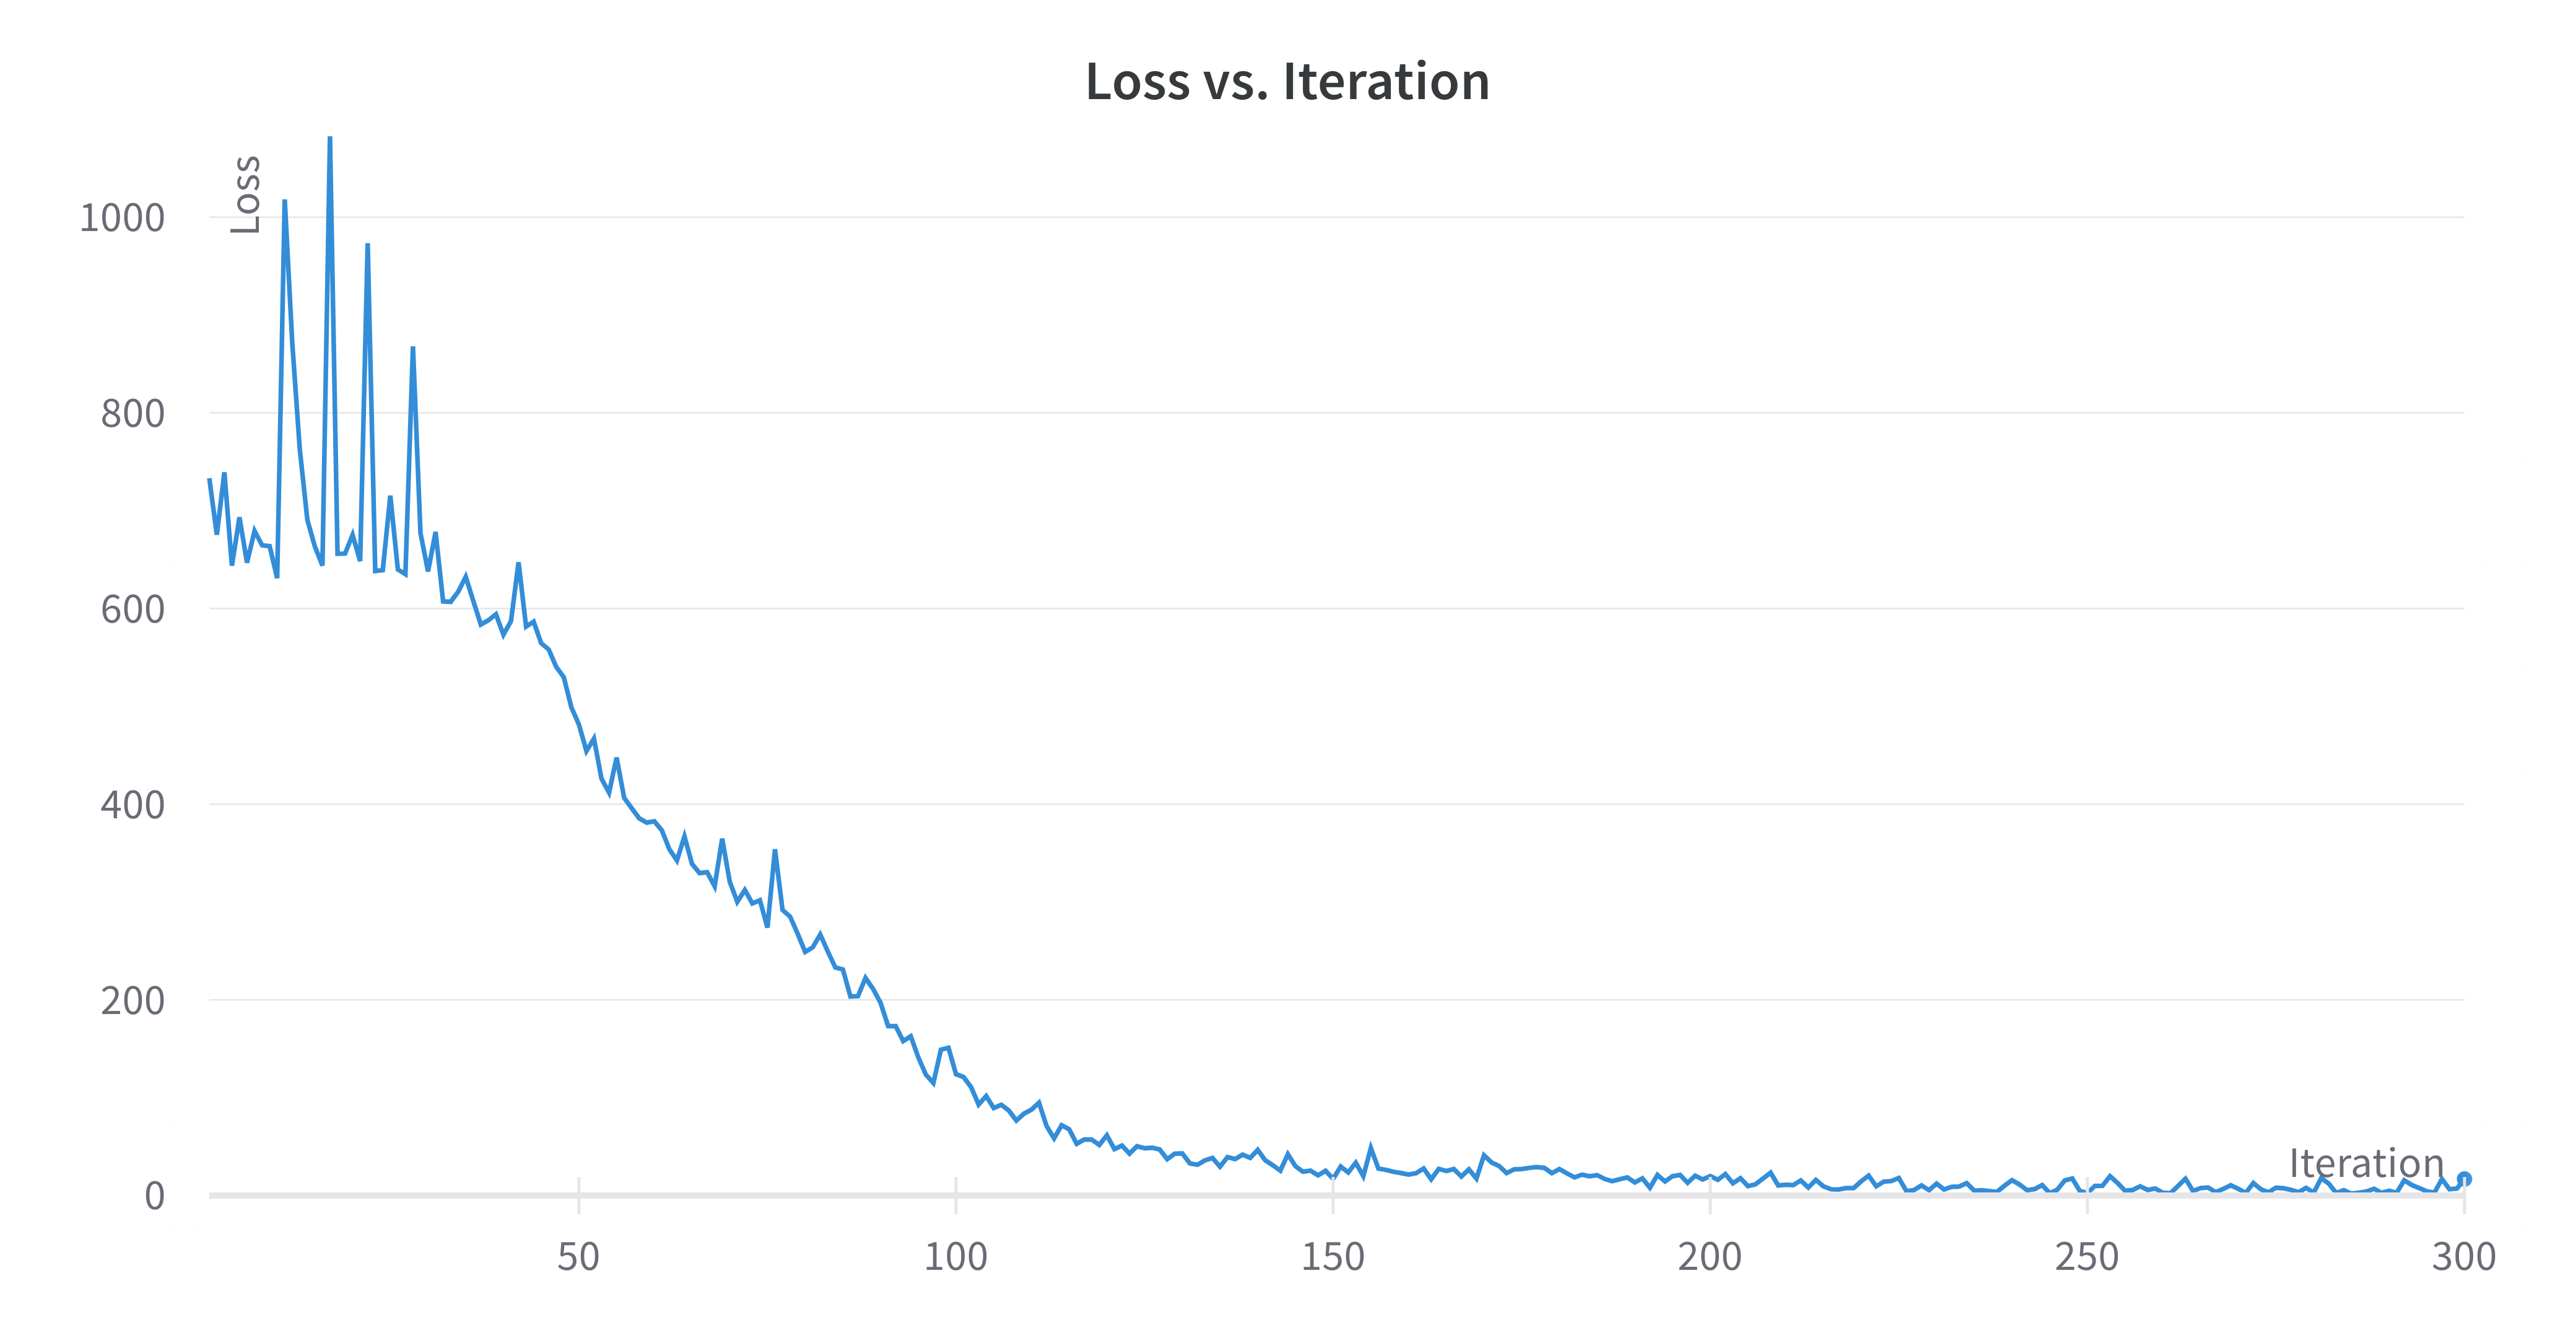
\includegraphics[width=0.6\textwidth]{images/attack_loss_iteration.png}
  \caption{CTC loss over 300 iterations of PGD.}
  \label{fig:attack_loss_iteration}
\end{figure}

\begin{figure}
  \centering
  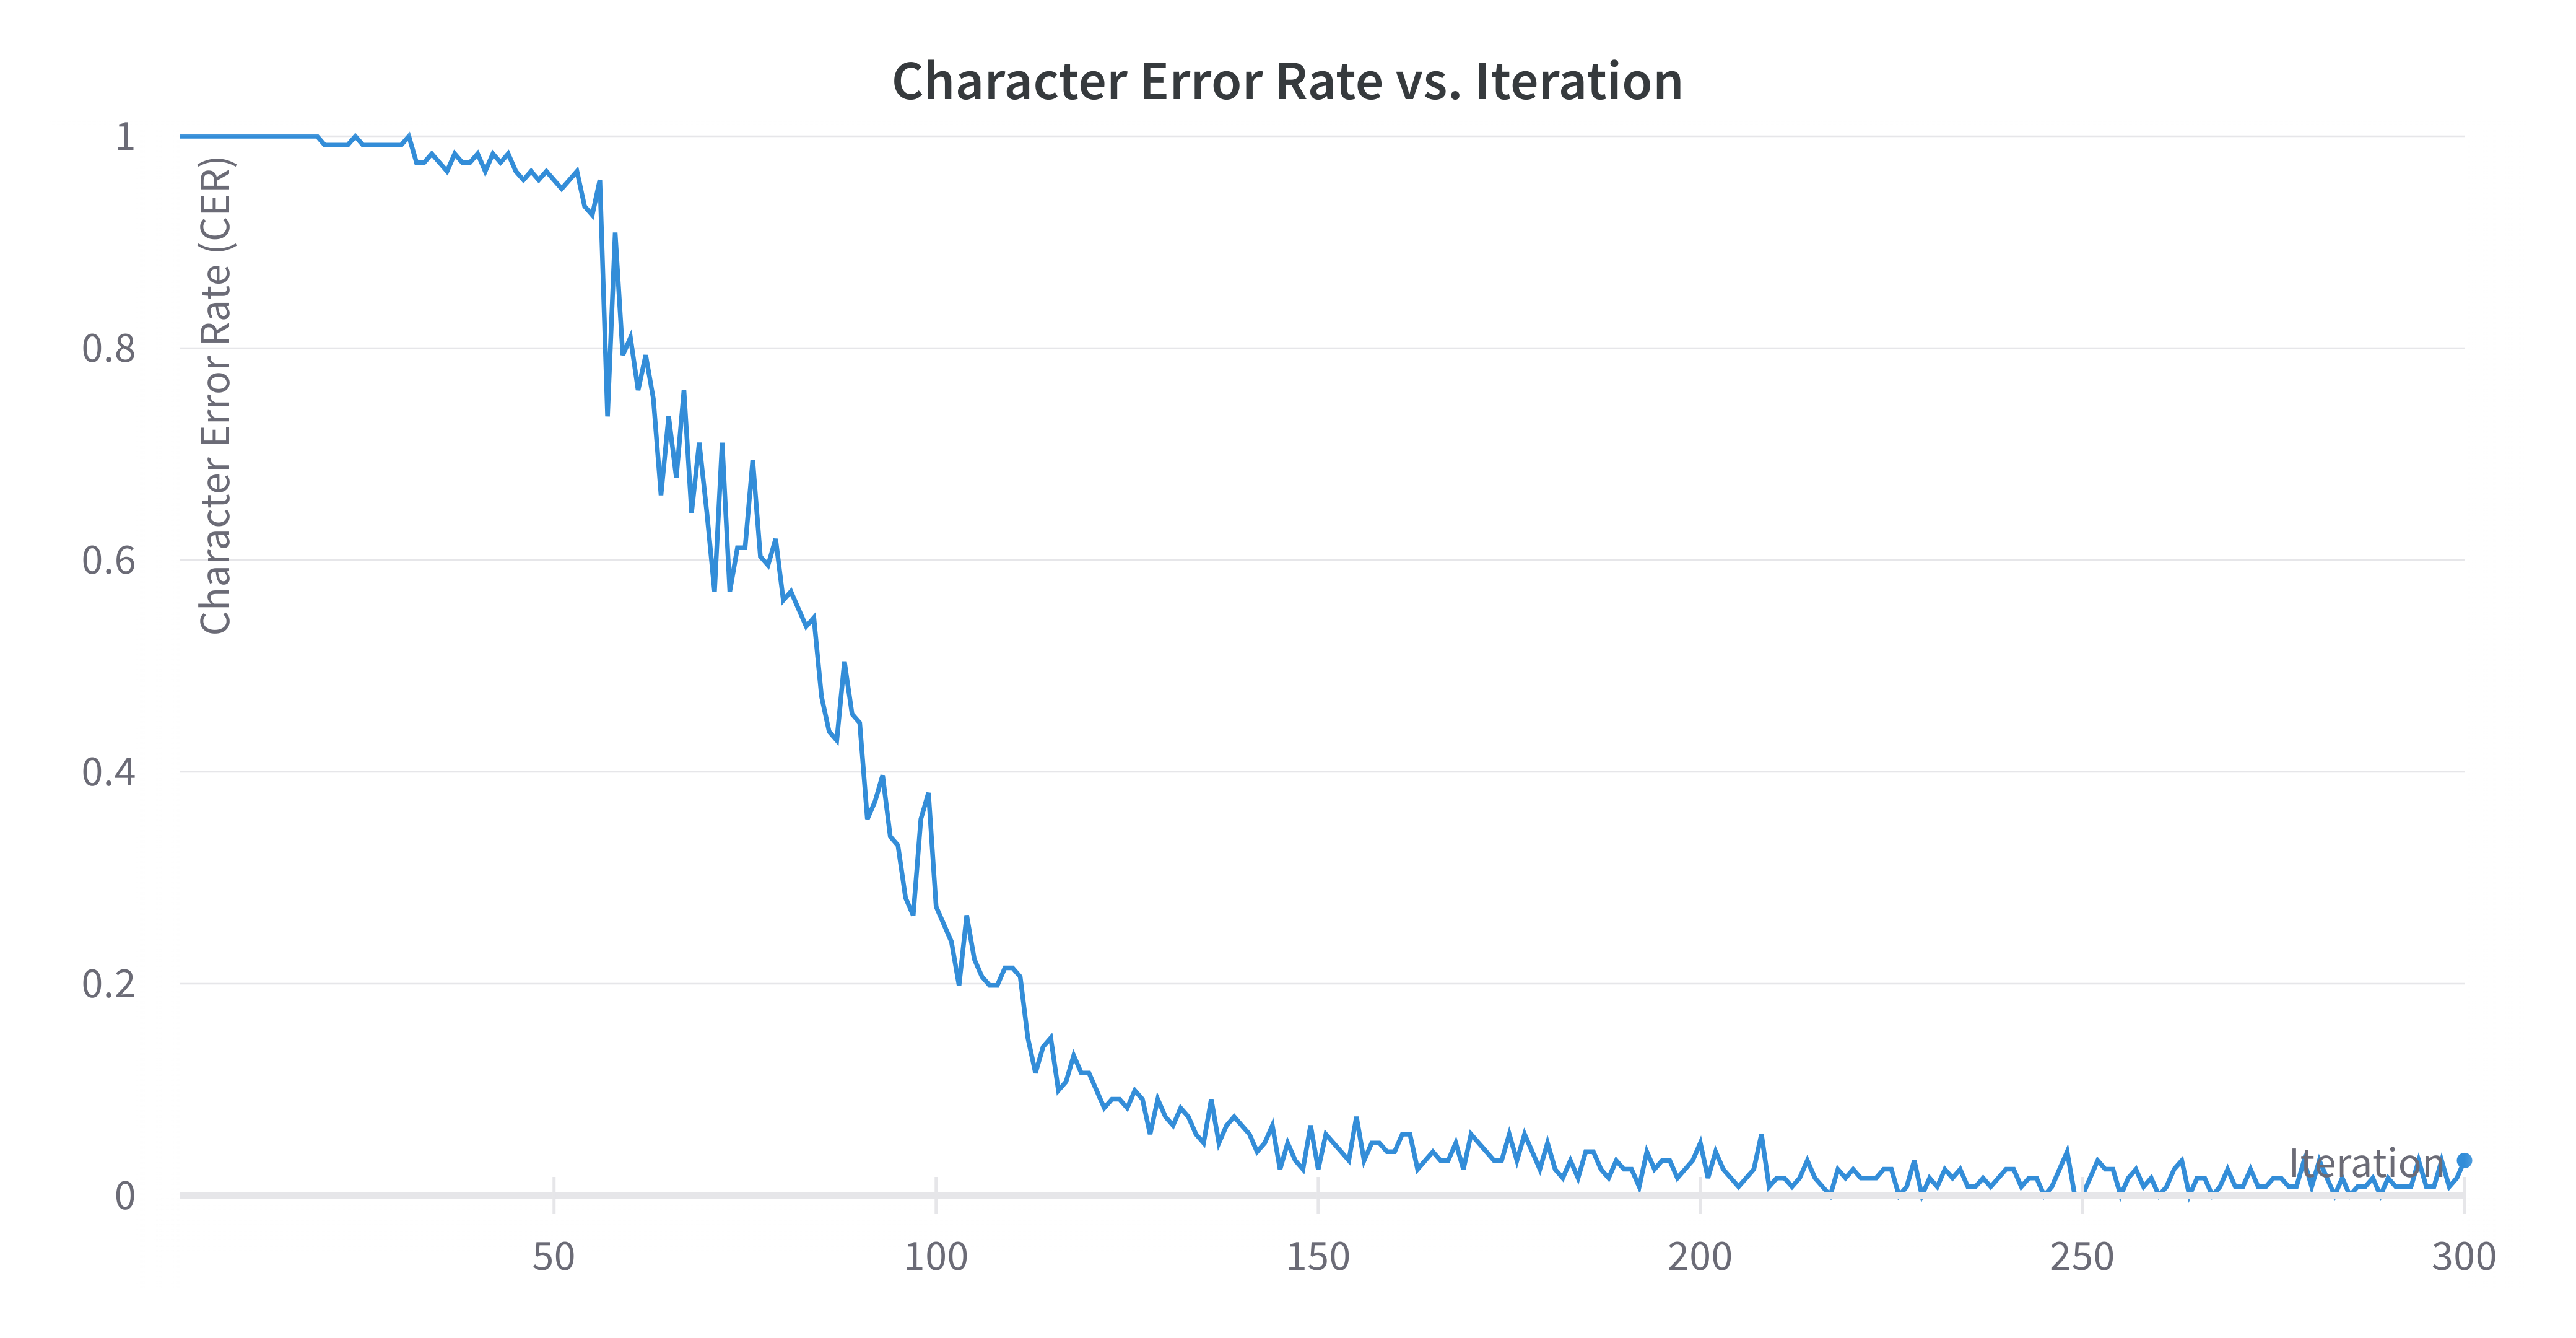
\includegraphics[width=0.6\textwidth]{images/attack_cer_iteration.png}
  \caption{CER over 300 iterations of PGD.}
  \label{fig:attack_cer_iteration}
\end{figure}

When we look at the transcripts generated by the speech recognition model at
various iterations of PGD (\autoref{tab:attack_transcript}), we see that even by
iteration 150, the adversarial transcript is quite close to the target
transcript. By iteration 250, only one word has a typo and by iteration 300, the
adversarial transcript is only off by one letter.

\begin{table}
  \centering
  \begin{tabularx}{\textwidth}{lX}
    \hline
    Iteration & Transcript \\
    \hline
    0         &            \\\\
    50        & \small\textbf{I} \textbf{CCON}     \\\\
    100       & \small\textbf{SEATTHE} \textbf{CENTE} \textbf{CKHAK} \textbf{TW} \textbf{THPEE} \textbf{LU} PIREP \textbf{TPEATUE} MINUS \textbf{UR} \textbf{COUD} \textbf{ASES} \textbf{THE} \textbf{THUAND} \textbf{HIGHT} \textbf{RN} \textbf{IC} \textbf{ACCATIN} \\\\
    150       & \small SEATTLE CENTER SKYHAWK TWO THREE ZULU PIREP \textbf{TEMPERAKTURE} \textbf{MAINUS} FOUR CLOUD BASES \textbf{THR} THOUSAND LIGHT RIME \textbf{KE} \textbf{ACCUMULATIN} \\\\
    200       & \small SEATTLE CENTER SKYHAWK TWO THREE ZULU PIREP \textbf{TEMPERARTURE} MINUS FOUR CLOUD BASES THREE \textbf{THTUSAND} LIGHT RIME ICE ACCUMULATION \\\\
    250       & \small SEATTLE CENTER SKYHAWK TWO THREE ZULU PIREP TEMPERATURE MINUS FOUR CLOUD BASES THREE THOUSAND LIGHT RIME \textbf{AKE} ACCUMULATION \\\\
    300       & \small SEATTLE CENTER SKYHAWK TWO THREE ZULU PIREP TEMPERATURE MINUS FOUR CLOUD BASES THREE THOUSAND LIGHT RIME ICE \textbf{ACCUMLATION} \\\\
    \hline
  \end{tabularx}
  \caption{Transcript of adversarial PIREP over 300 iterations of PGD. Words with typos are bolded.}
  \label{tab:attack_transcript}
\end{table}

Another interesting visualization of our method is the spectrogram of the intial
noise selected from \autoref{eq:noise} compared to the adversarial PIREP after
300 iterations of PGD (\autoref{fig:spectrograms}). In the bottom spectrogram,
we can visually see the result of our adversarial attack in the form of a
distinct pattern in the 0 to 3000 Hz frequency range. Although this pattern can
be seen on the spectrogram, it is not easily detectable by the human ear over
the static noise.

\begin{figure}
  \centering
  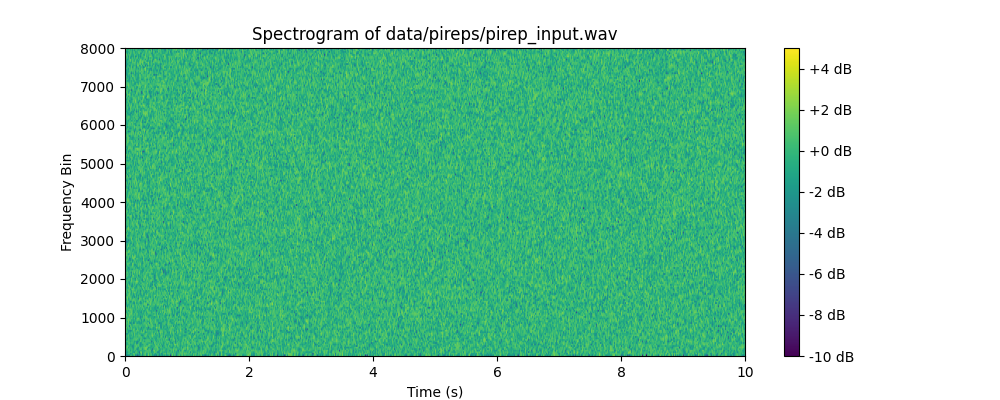
\includegraphics[width=0.8\textwidth]{images/pirep_input.png}
  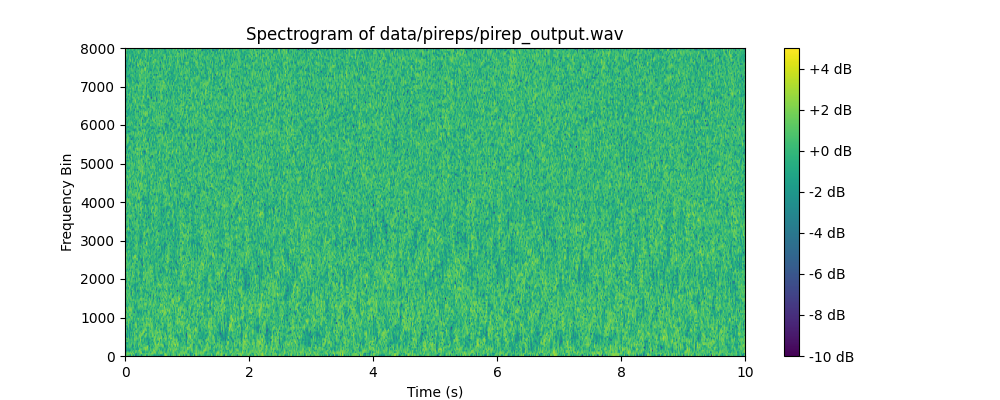
\includegraphics[width=0.8\textwidth]{images/pirep_output.png}
  \caption{\textit{Top}: Spectrogram showing randomly selected noise from \autoref{eq:noise}. \textit{Bottom}: Spectrogram showing adversarial PIREP after 300 iterations of PGD. Notice the formations in the 0 to 3000 Hz frequency range.}
  \label{fig:spectrograms}
\end{figure}

\section{Evaluation}

\subsection{Static Consequences}

Static interference poses significant challenges for flight traffic controllers
when it comes to radio communication. This interference, often caused by
atmospheric conditions or electromagnetic disturbances, can result in distorted
or garbled transmissions, making it difficult for controllers to receive and
interpret crucial information from pilots. Static interference can lead to
miscommunication, misunderstandings, and delays in coordinating flight
operations. This posses a problem for our attack vector, if sufficient static is
introduced into the system it can cause our attack to fail.

\subsection{Noise Injection}
\label{sec:noise_injection}

% \begin{figure}
%   \centering
%   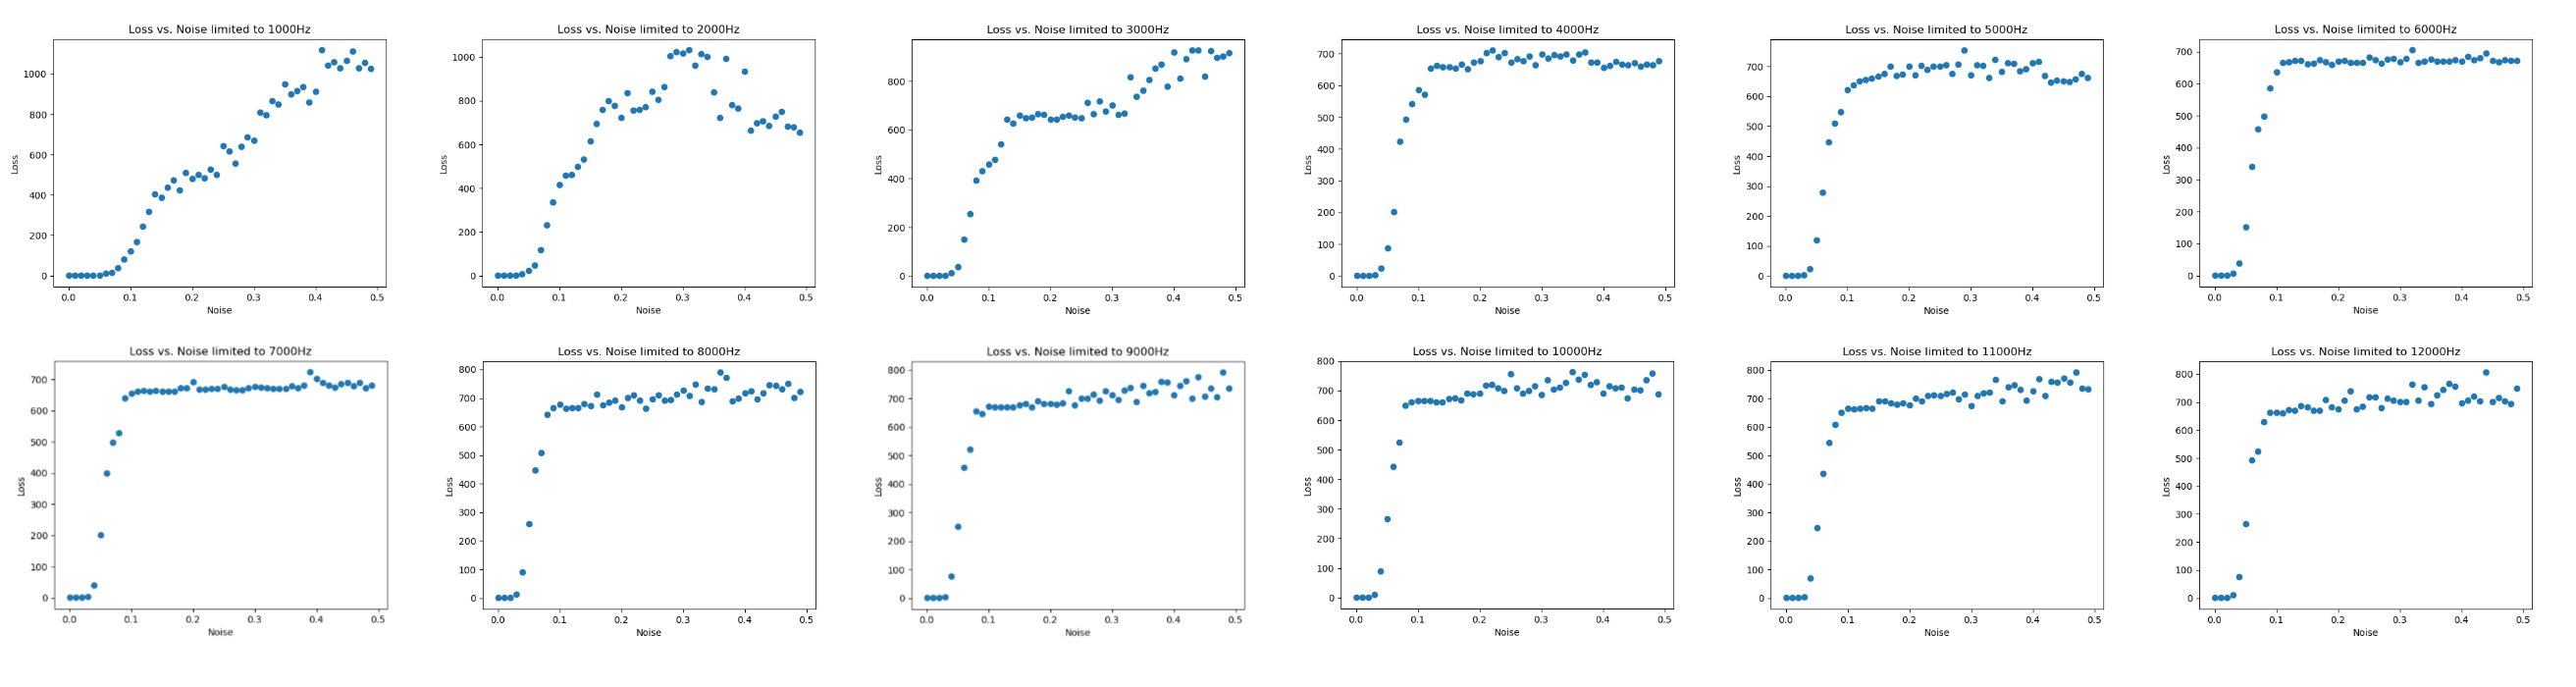
\includegraphics[width=1.0\textwidth]{images/Loss_vs_Noise_bandwidth_low_to_high_HD.png}
%   \caption{The graph illustrates the relationship between the loss to noise ratio and the incremental increase of noise in 1000 hertz intervals, extending up to a maximum value of 12000 hertz.}
%   \label{fig:loss_vs_noise_low_to_high}
% \end{figure}

\begin{figure}
  \centering
  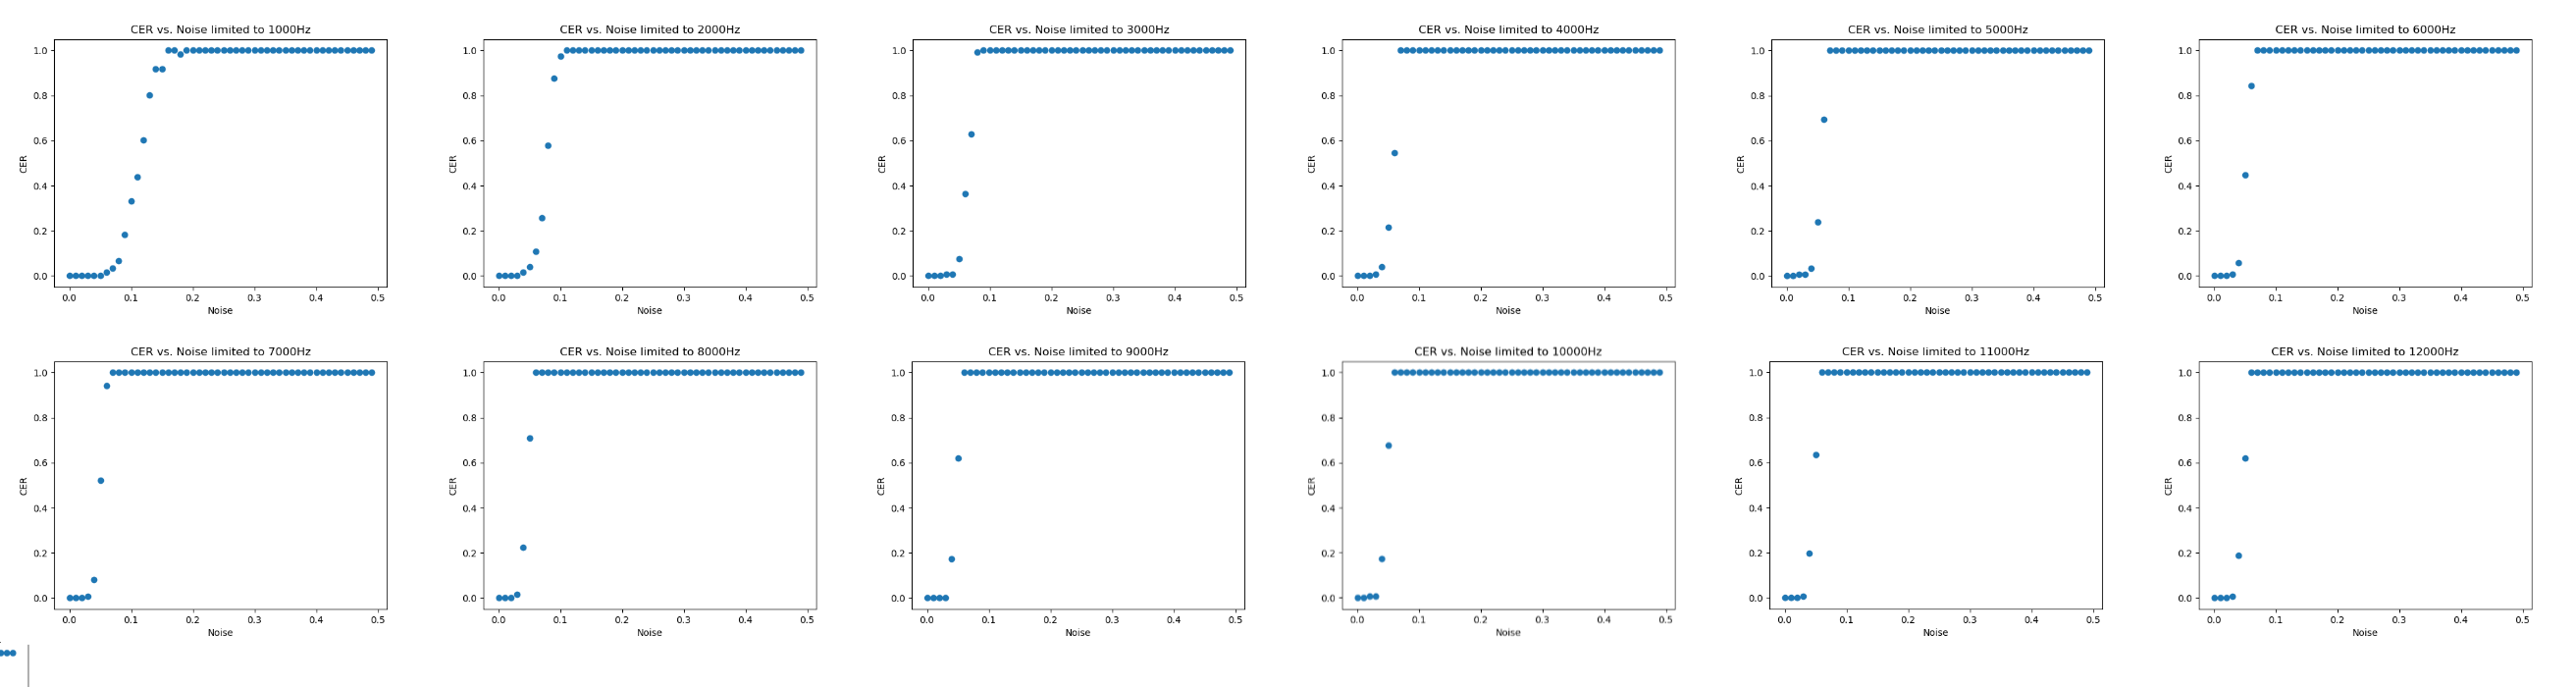
\includegraphics[width=1.0\textwidth]{images/CER_vs_Noise_bandwidth_low_to_high_HD.png}
  \caption{The graph showcases the correlation between the CER and the incremental rise of noise in 1000 hertz intervals, reaching a maximum value of 12000 hertz.}
  \label{fig:cer_vs_noise_low_to_high}
\end{figure}

\begin{figure}
  \centering
  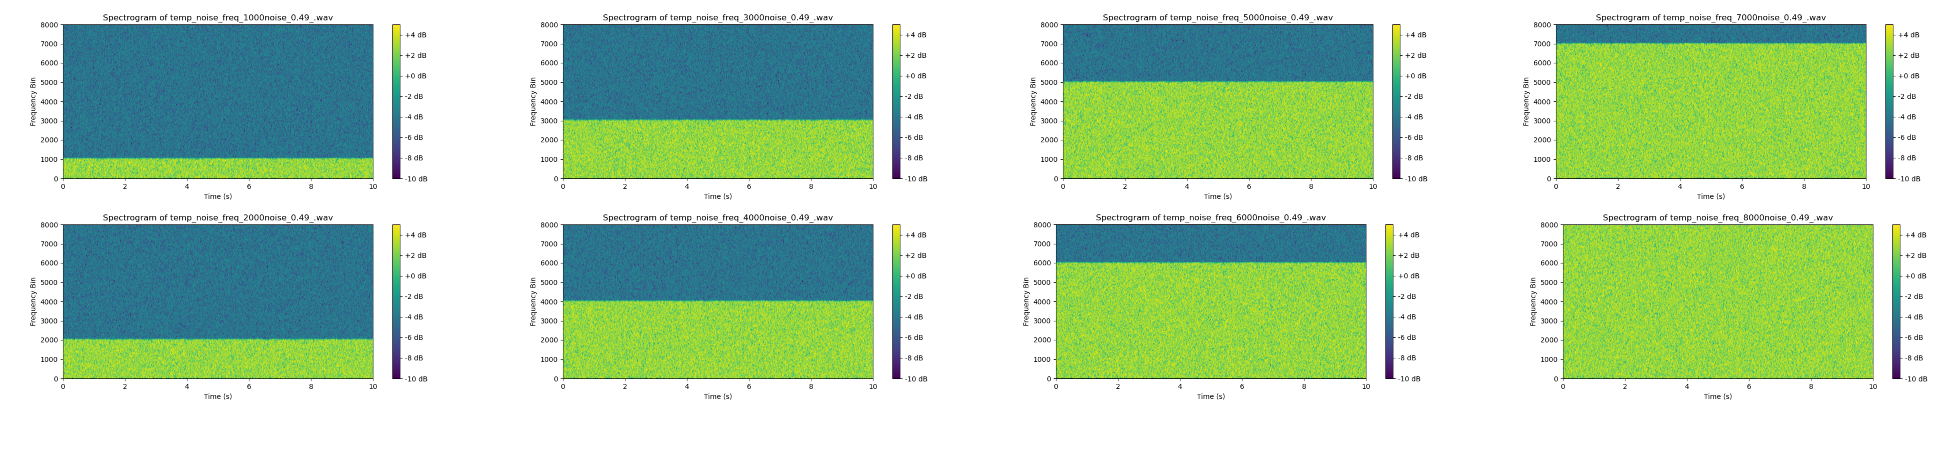
\includegraphics[width=1.0\textwidth]{images/spectrograms_low_to_high.png}
  \caption{These spectrographs demonstrate the noise that was applied to the two above figures for the values of 1000 hertz to 8000 hertz, with increments of 1000 hertz.}
  \label{fig:spectrograms_low_to_high}
\end{figure}

The outcomes depicted in \autoref{fig:cer_vs_noise_low_to_high} showcase the
impact of progressively increasing noise from a frequency range of 1000 Hz to
12000 Hz. These figures also demonstrate the corresponding CER for our example
of an adversarial attack. The findings imply that as the frequency at lower
hertz rate increase the observed loss rate and CER rate increase. Additionally,
\autoref{fig:spectrograms_low_to_high} displays the spectrograms of the noise
files utilized to perturb the adversarial static audio.

Upon analyzing these figures, a clear trend emerges. As the frequency at lower
hertz rates increases, there is a noticeable rise in CER. In other words, when
the noise introduced to the system falls within the lower frequency range, it
leads to a greater degree of distortion and inaccuracy in the audio. This
finding suggests that the adversarial attack is less potent and capable of
causing significant disruptions when the noise contains lower frequency
components.

% \begin{figure}
%   \centering
%   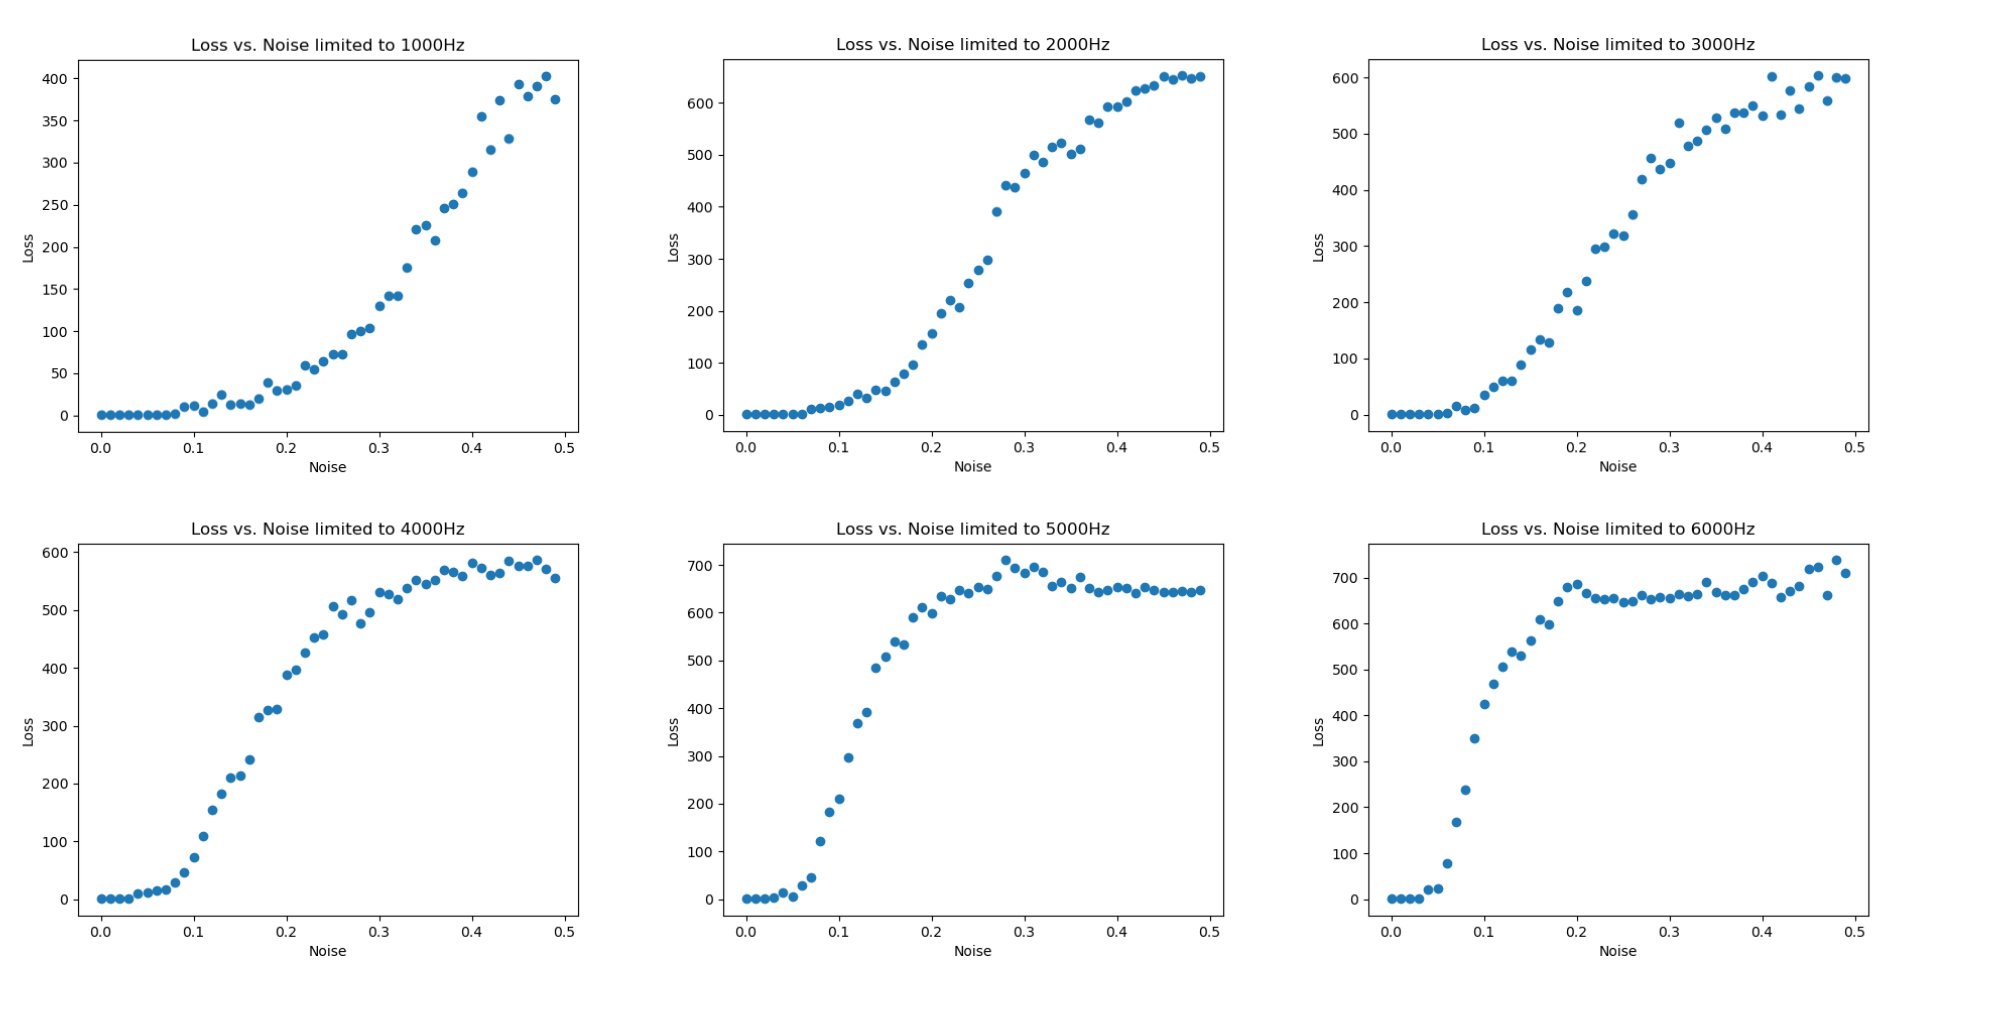
\includegraphics[width=1.0\textwidth]{images/Loss_vs_Noise_bandwidth_high_to_low_HD.png}
%   \caption{The graph depicts the correlation between the loss to noise ratio and the gradual escalation of noise from 8000 hertz to 1000 hertz, with increments of 1000 hertz.}
%   \label{fig:loss_vs_noise_high_to_low}
% \end{figure}

\begin{figure}
  \centering
  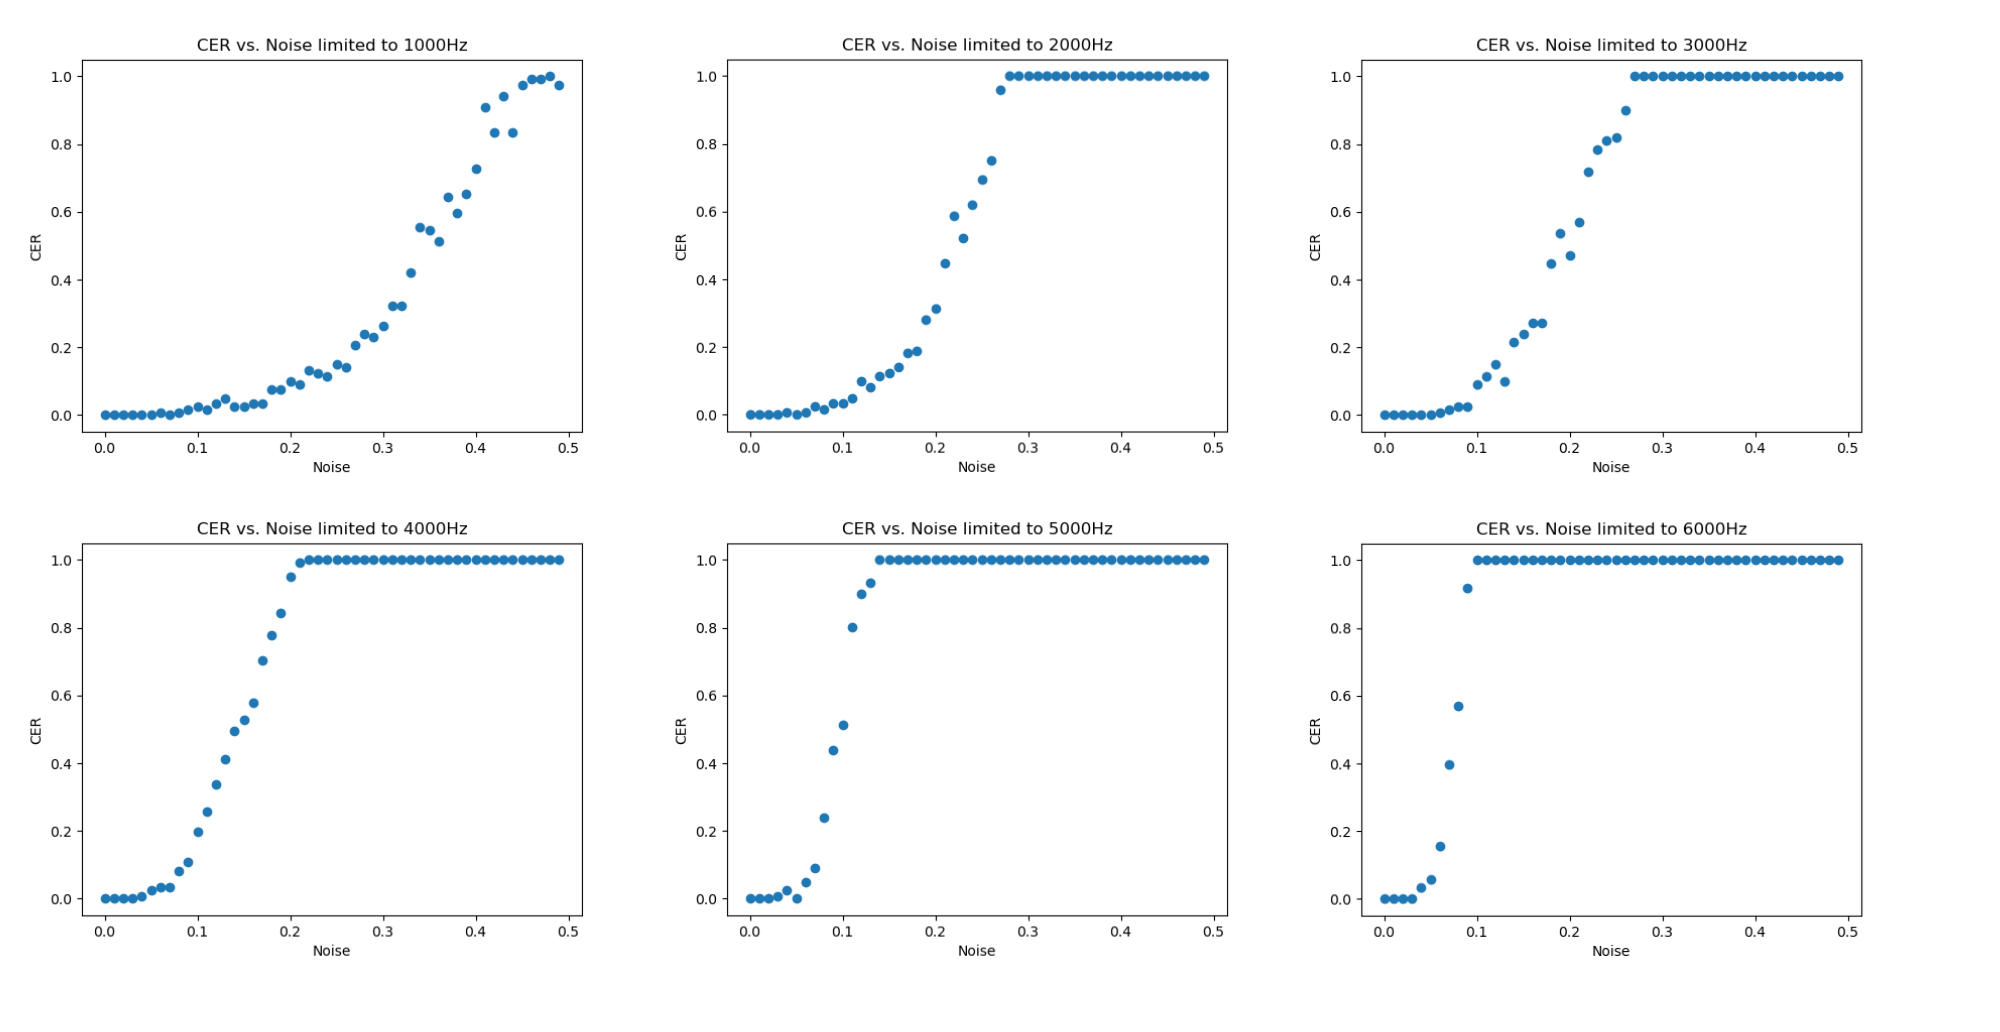
\includegraphics[width=1.0\textwidth]{images/CER_vs_Noise_bandwidth_high_to_low_HD.png}
  \caption{The graph illustrates the relationship between the CER to noise ratio and the progressive increase of noise from 8000 hertz to 1000 hertz, with increments of 1000 hertz.}
  \label{fig:cer_vs_noise_high_to_low}
\end{figure}

\begin{figure}
  \centering
  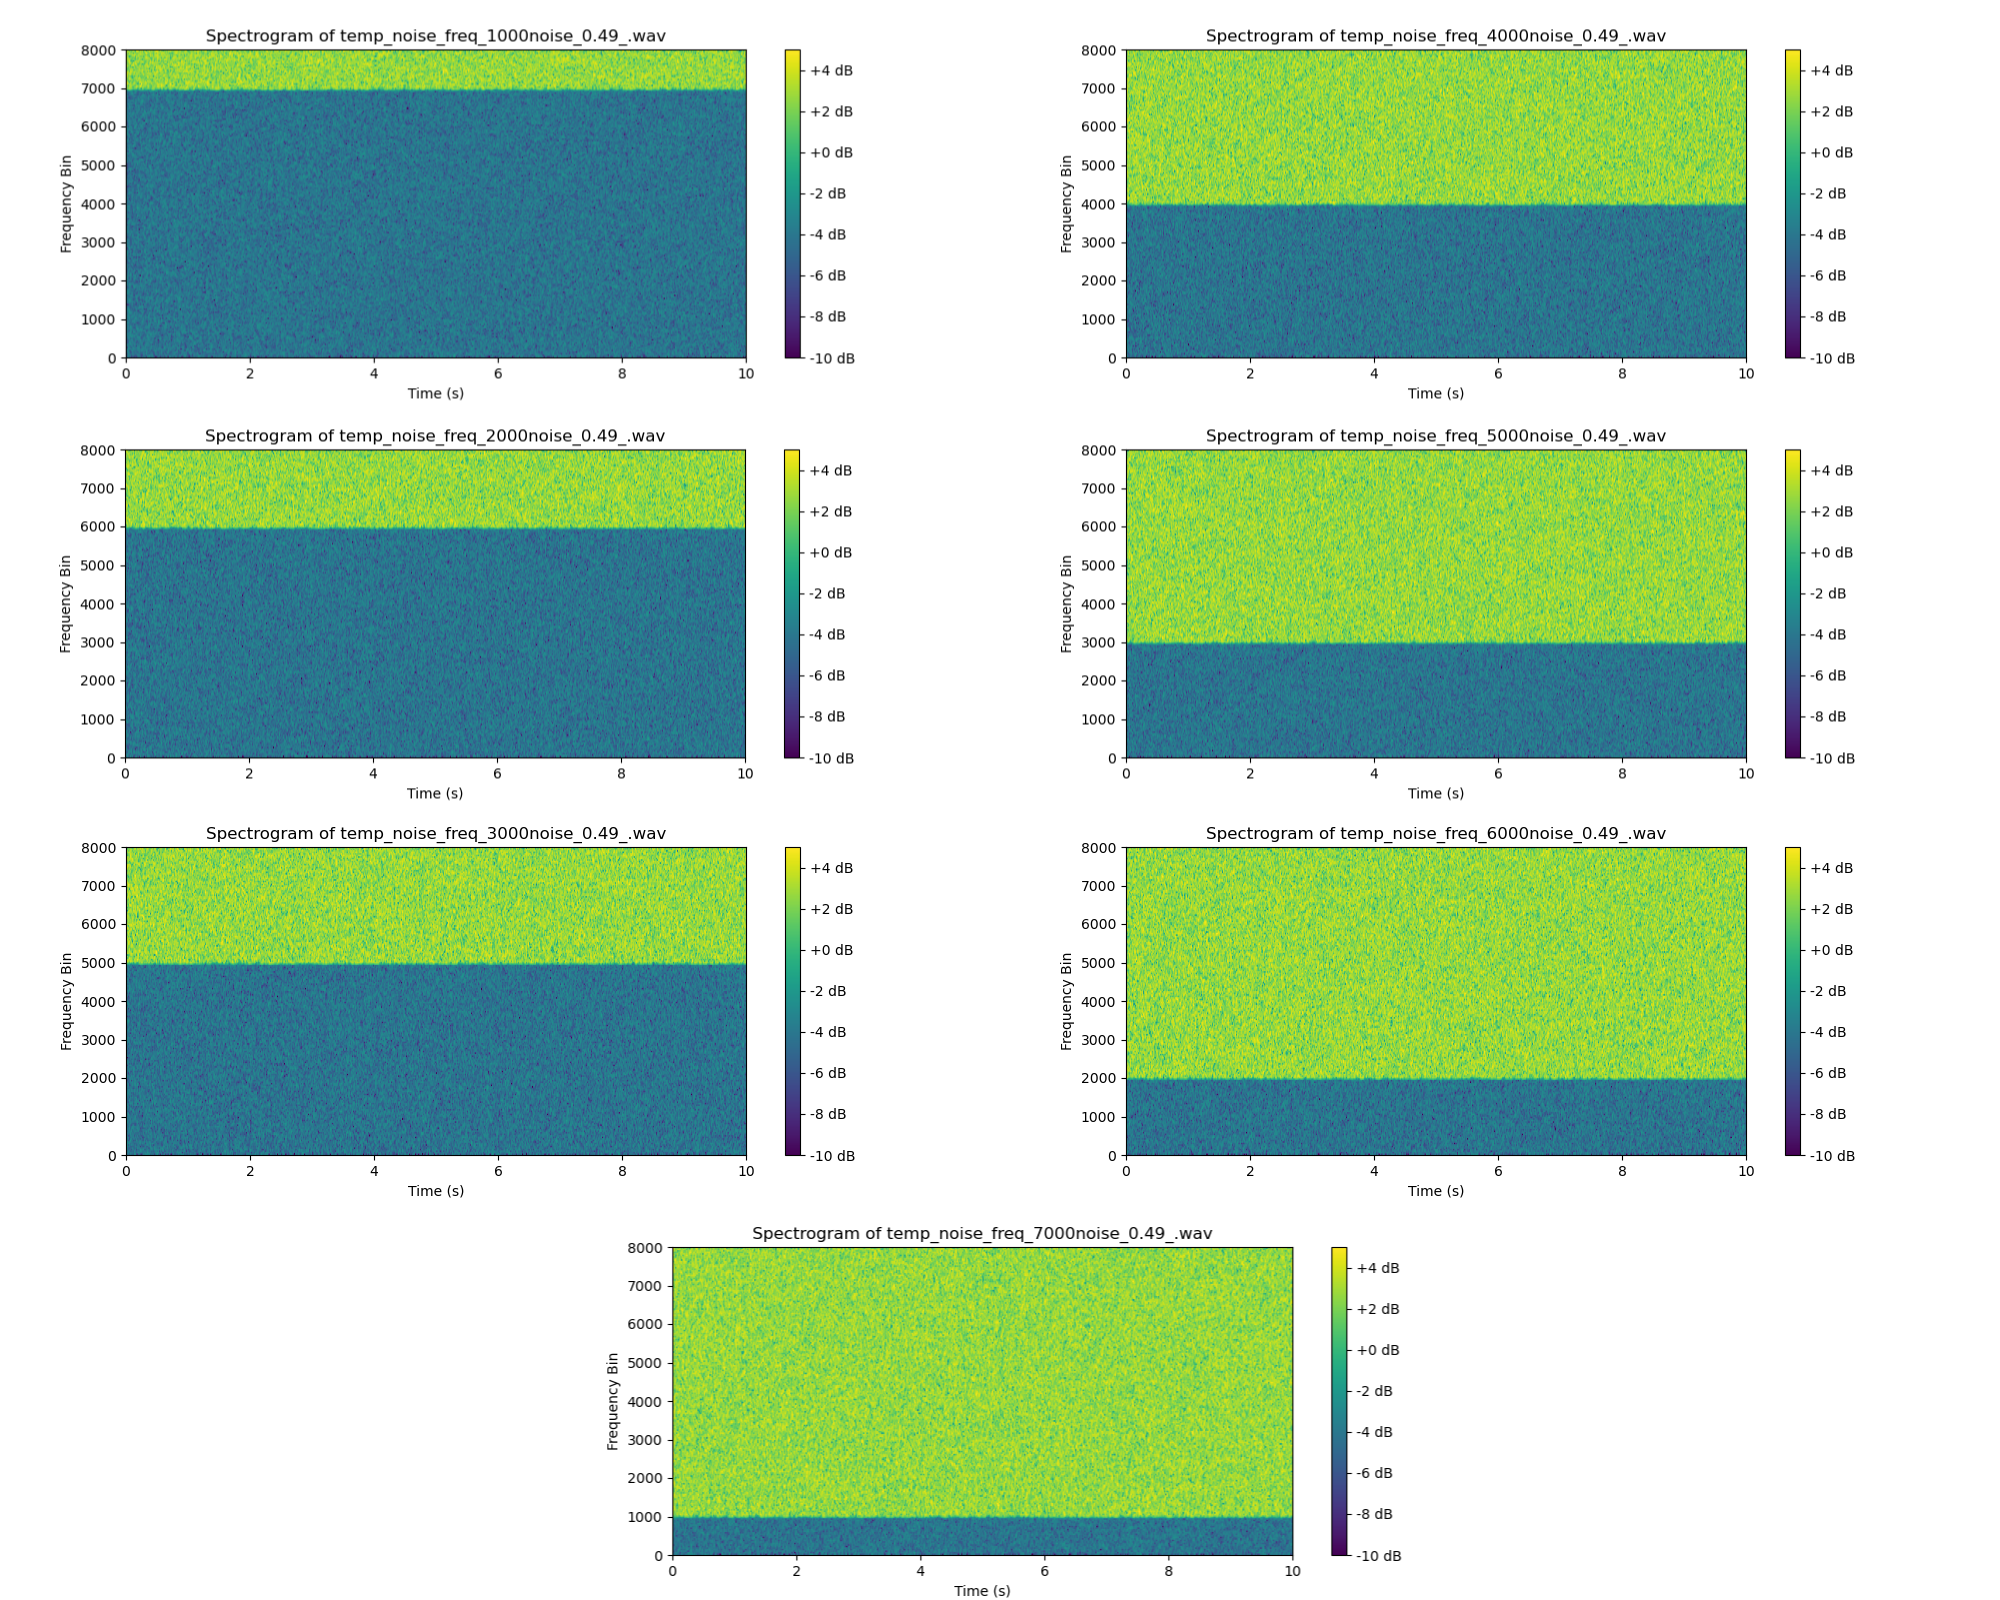
\includegraphics[width=1.0\textwidth]{images/spectrograms_high_to_low.png}
  \caption{These spectrographs demonstrate the noise that was applied to the two above figures for the values of 8000 hertz to 1000 hertz, with increments of 1000 hertz.}
  \label{fig:spectrograms_high_to_low}
\end{figure}

The results shown in \autoref{fig:cer_vs_noise_low_to_high} provide evidence of
a more pronounced impact compared to the outcomes depicted in \autoref{fig:cer_vs_noise_high_to_low}.
In \autoref{fig:cer_vs_noise_low_to_high}, it is observed that the
high-frequency noise eventually eliminates the adversarial attack, but in
and \autoref{fig:cer_vs_noise_high_to_low} this process requires significantly
more time and effort.

It becomes evident that the introduction of high-frequency noise is capable of
eventually eradicating the adversarial attack. However, this process requires a
significantly longer duration and greater intensity of noise. The gradual
escalation of high-frequency noise is observed to have a slower and more gradual
effect on the loss rate and CER rate

\begin{figure}
  \centering
  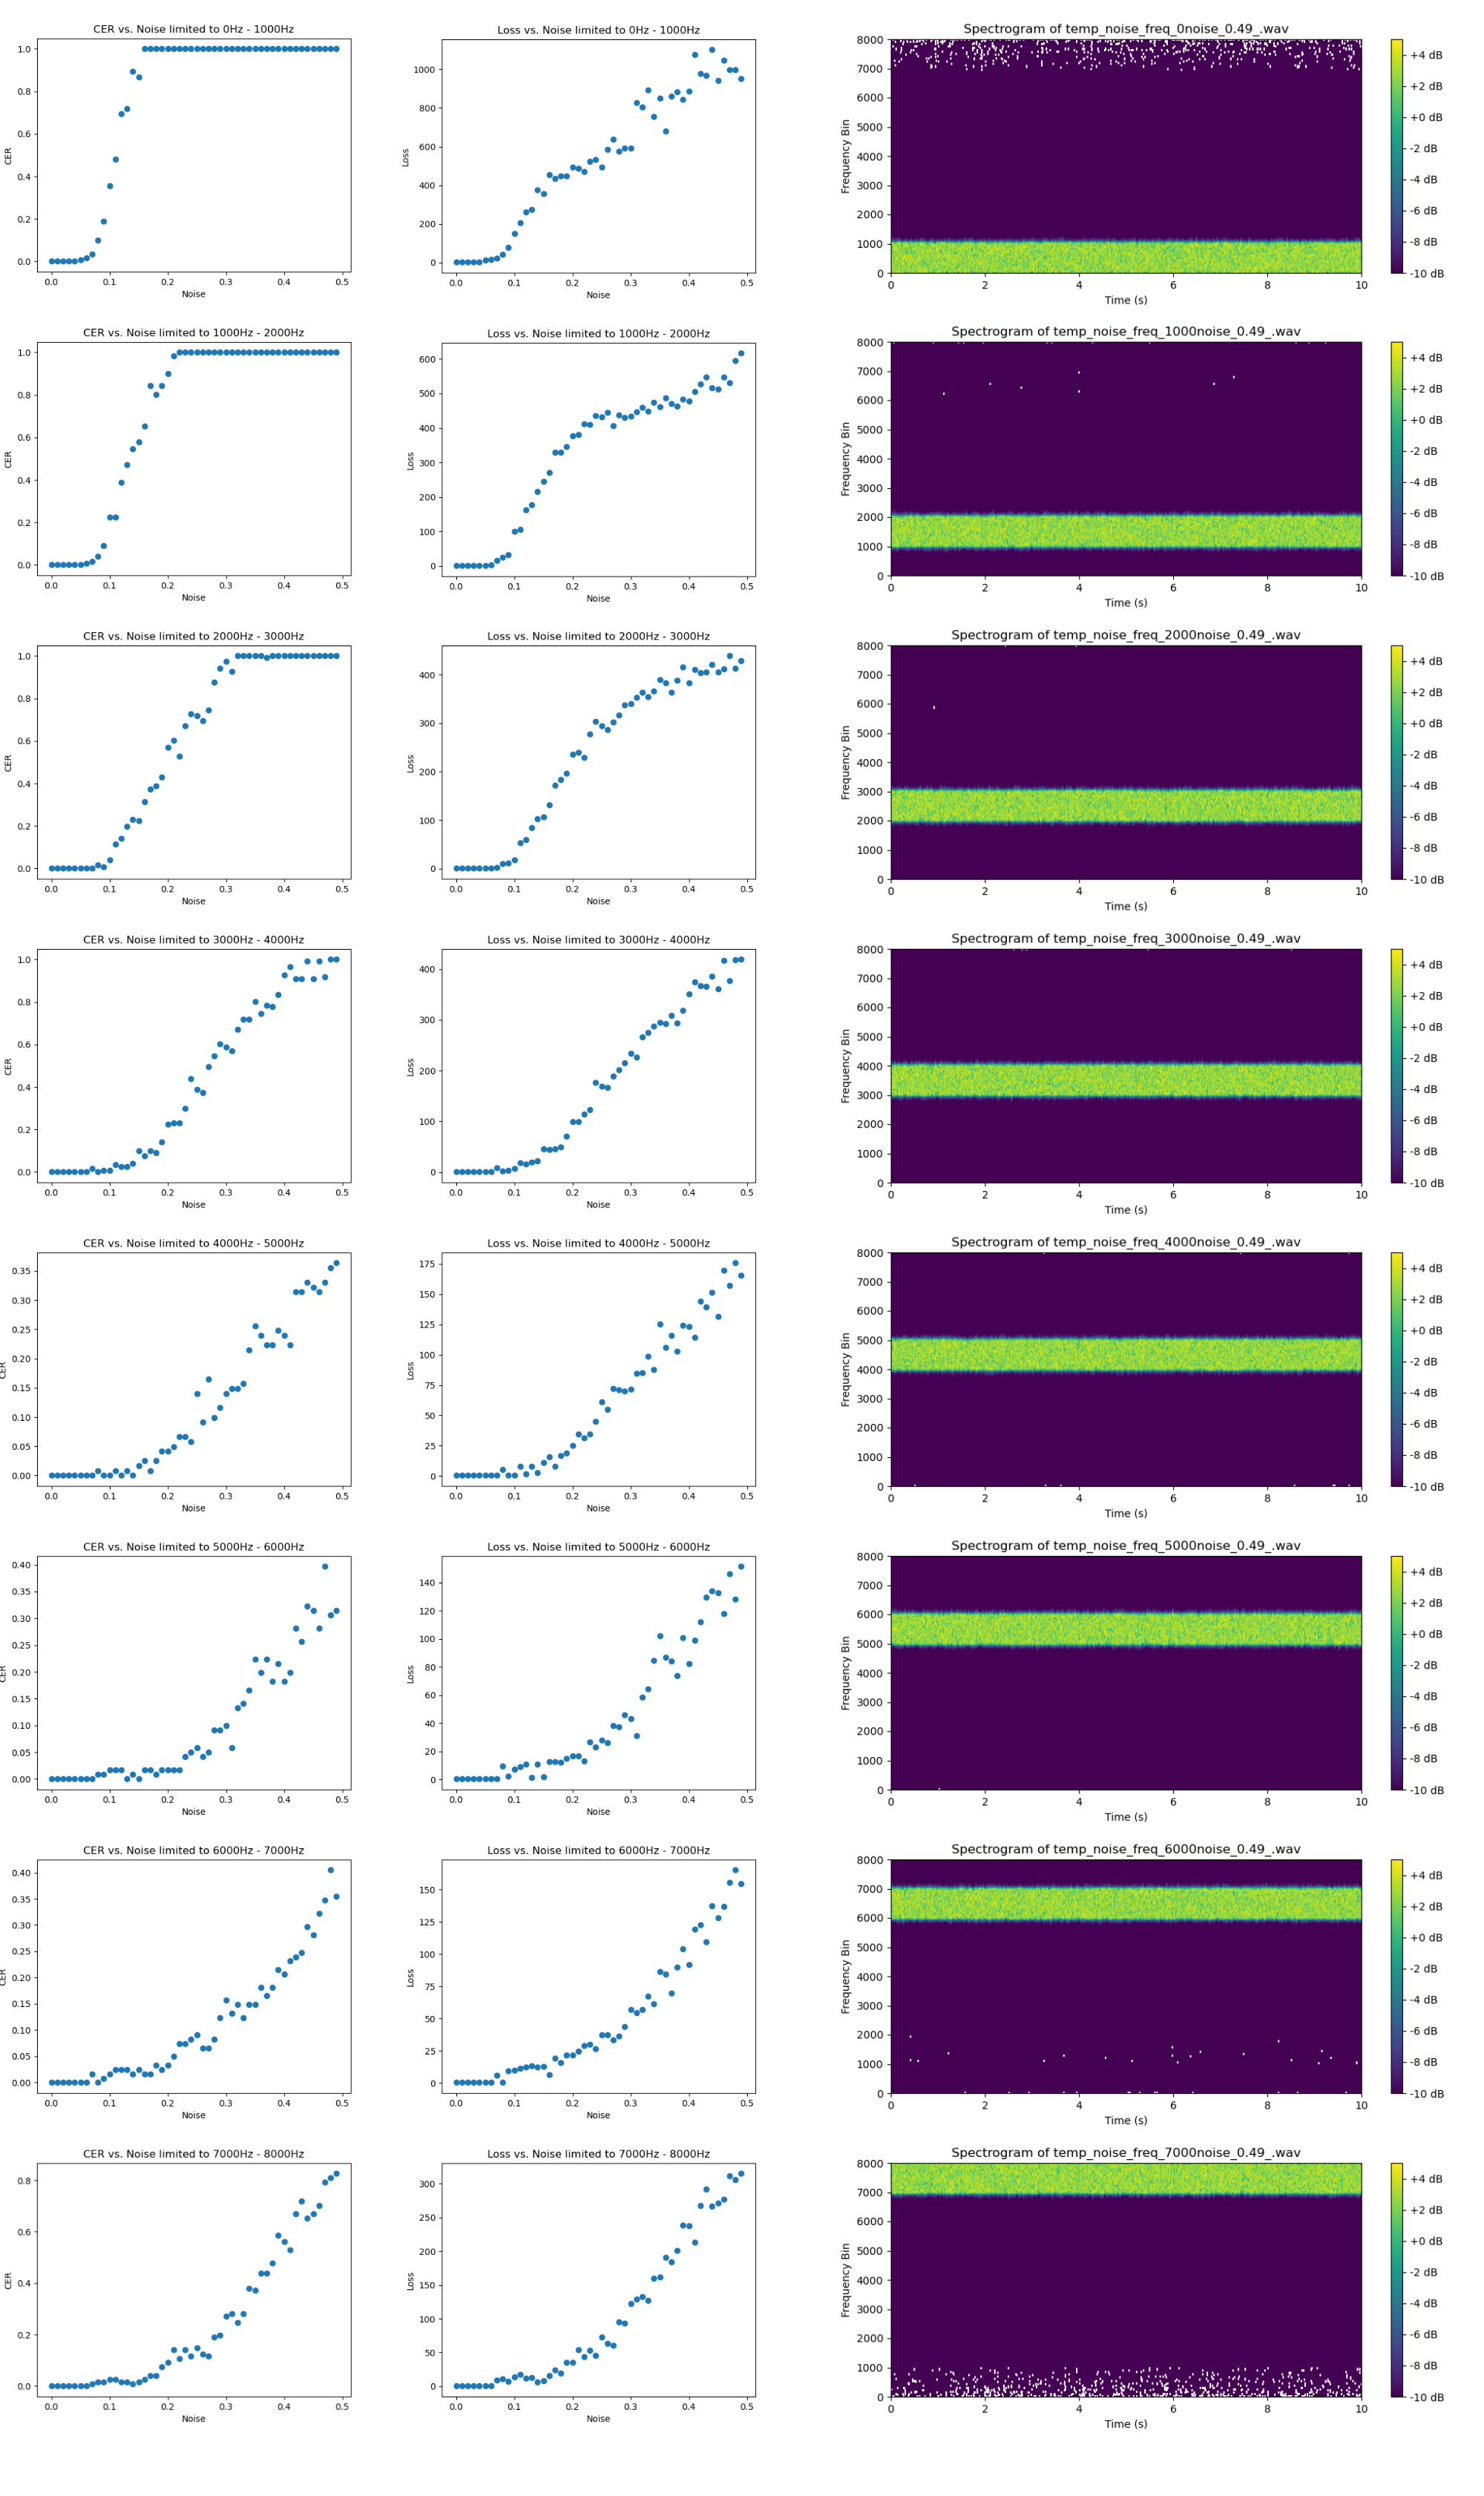
\includegraphics[width=0.8\textwidth]{images/WaveBandTestingStatic.png}
  \caption{The figure should be read from left to right starting at the top and proceeding downward for each new test. Each row represents a different test with 3 data graphs per test. From left to right they are CER vs Noise, Loss vs Noise, spectrograms representation of the noise applied to the adversarial attack.}
  \label{fig:WaveBandTestingStatic}
\end{figure}

After conducting tests involving the escalation of noise from low frequency
ranges to high frequency ranges and vice versa, our next objective was to
determine the specific bands of static that have the most impact on our
adversarial attack. Through careful analysis of the results obtained, we have
reached a conclusion: the low frequency bands ranging from 0 to 2000 hertz have
the most significant influence on our perturbed attack.

These findings indicate that the introduction of noise within the lower
frequency range has a particularly detrimental effect on the integrity and
intelligibility of the attacked message. The distortions caused by the static
within these specific frequency bands lead to a higher degree of disruption and
distortion, significantly impacting the attack's success.

However, it is important to note that while the low frequency bands have the
most pronounced impact, the results show that all frequency bands eventually
contribute to the degradation of the attacked message. Regardless of the
specific frequency range, the cumulative effect of the noise causes the CER to
reach approximately 70 precent, meaning that the original message becomes
distorted to the point of being unrecognizable or unintelligible.

\begin{figure}
  \centering
  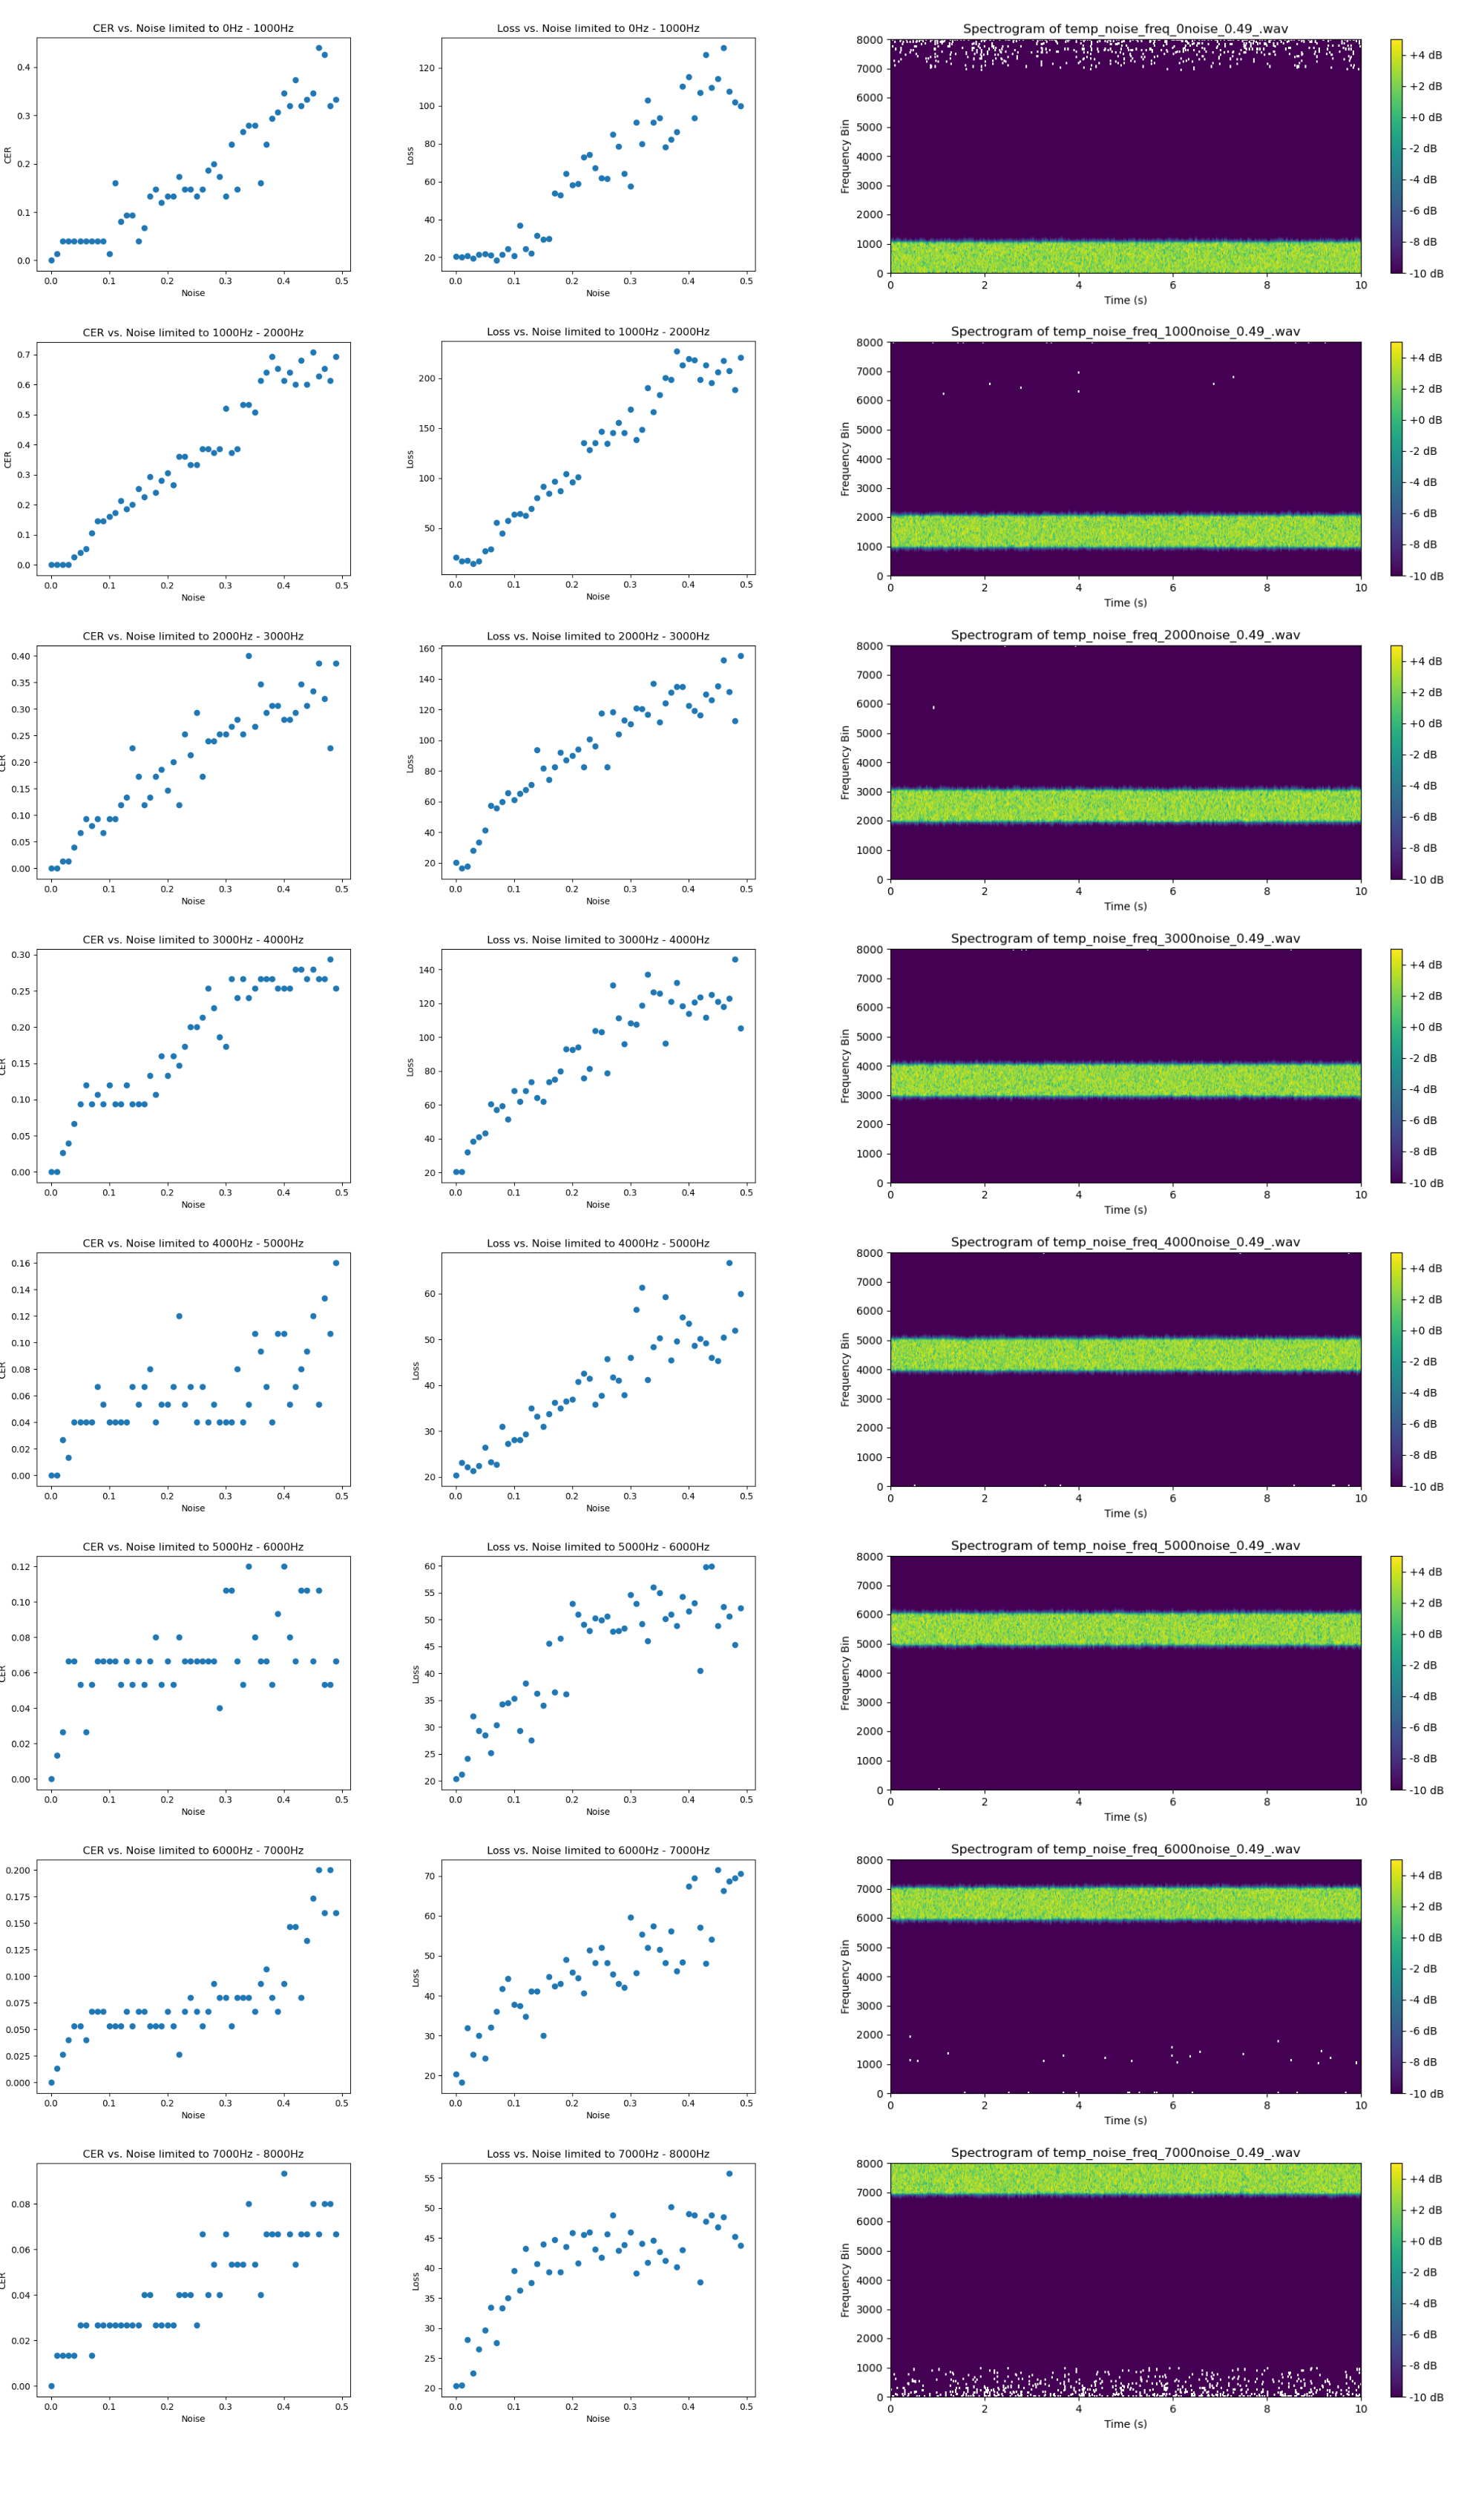
\includegraphics[width=0.8\textwidth]{images/WaveBandTestingRegularAudio.png}
  \caption{The figure should be read from left to right starting at the top and proceeding downward for each new test. Each row represents a different test with 3 data graphs per test. From left to right they are CER vs Noise, Loss vs Noise, spectrograms representation of the noise applied to the normal audio with speech.}
  \label{fig:WaveBandTestingRegularAudio}
\end{figure}

In a similar vein, when conducting tests on regular audio without any
perturbations, we discovered similar trends within the 0-3000 hertz frequency
range. However, the outcomes exhibited distinct characteristics when compared to
the results obtained from the adversarial attack scenario.

Within the regular audio context, the findings demonstrated that at higher
frequencies, specifically in the range of 5000-8000 hertz, there wasn't a
notable loss of audio information. This loss resulted in a relatively low CER
range of 0.08 to 0.30, indicating that the audio remained highly legible and
intelligible to machine learning audio recognition software.

\subsection{Static Findings}

The analysis of frequency bands in both the adversarial attack and regular audio
scenarios yielded valuable insights. In the adversarial attack scenario and
regular audio without perturbations, low frequency bands (0-2000 hertz) had the
most significant impact on the audio, while all frequency bands contributed to
the overall degradation of the attacked message. Conversely, in regular audio
without attack perturbations, higher frequencies (5000-8000 hertz) did not
greatly affect the machine learning algorithms ability to translate the audio
file.

\section{Defenses}

there are several methods for defending against our adversarial PIREPs. These
methods are proposed as a starting point for future research, and should be
evaluated in real-world settings before being deployed in safety-critical
systems.

\subsection{Defensive Noise Injection}

One unconventional yet basic defense mechanism against static attacks involves
injecting noise specifically in the frequency range of 7000-8000 hertz, using an
epsilon value of 0.5. This defense strategy intentionally degrades the regular
audio, resulting in a CER degradation of approximately 0.08. This defense
approach mostly eliminates the adversarial attack, rendering it unrecognizable.

Within the regular audio context, the findings demonstrated that at higher
frequencies, specifically in the range of 7000-8000 hertz, there was not a
notable loss of audio information. This loss resulted in a relatively low CER
range of 0.08 to 0.30, indicating that the audio remained highly legible and
intelligible to machine learning audio recognition software.

\subsection{Adversarial Detection Model}

An alternative approach to detecting static audio is employing multiple models
with different architectures to analyze the audio data. This method involves
flagging instances where the interpretations of these distinct models differ
significantly. However, implementing this approach poses certain challenges,
particularly in the aviation domain where specialized audio recognition software
models tailored for specific flight control language would be necessary.

One potential solution is combining a regular speech detection model with a
sophisticated flight control model. By utilizing both models in tandem, it may
become possible to detect static communications that has been picked up by one
model but not the other. This complementary approach enhances the overall
detection capability and is possible to increase the likelihood of accurately
identifying static audio.

It is important to note that integrating multiple models and specialized
software comes with its own set of complexities. Building and maintaining such
models requires domain expertise, extensive training data, and continuous
refinement to ensure their effectiveness in detecting static audio.

\subsection{Gradual Implementation}

Finally, one of the simplest and most effective defenses against adversarial
attacks is a human in the loop. In the case of PIREPs, this may mean that an air
traffic controller would be responsible for reviewing the PIREP before it is
entered into the system. This would be a simple and effective defense against
our attack since a human would be able to easily classify the adversarial PIREP
as static. Although this does require additional effort from the air traffic
controller, it would likely still be less work than the current process of
transcribing the PIREP by hand, and thus still helpful in reducing the workload
of air traffic controllers.

\section{Conclusion}

This paper introduces a novel adversarial attack specifically designed for speech
recognition systems utilized in air traffic control settings. Our attack is able to
successfully fool a state-of-the-art speech recognition model (Wav2Vec 2.0) into
transcribing static as a valid PIREP. We also evaluate the robustness of our
attack to various types of noise\textemdash simulating transmission over
radio\textemdash and find that the robustness heavily depends on the frequency
range of the noise. Finally, we propose several defenses against our attack,
including injecting noise in the frequency range of 7000-8000 hertz and using
multiple models to detect adversarial examples prior to transcription. Perhaps
most importantly, we suggest that the FAA should consider initially deploying
their system with a human in the loop, as this would be a simple and effective
defense against our attack, while still providing significant benefits to air
traffic controllers compared to the current process of transcribing PIREPs by
hand.

\subsection{Future Work}

Improvements to our attack could be made by using various alternative methods.
For example, we could use a variant of psychoacoustic hiding
\cite{schonherr2018adversarial} to hide the adversarial example in frequency
ranges that are less likely to be affected by static interference (as
investigated in \autoref{sec:noise_injection}). Such a model would be more
robust to static interference, and thus more likely to be successful in a
real-world setting.

Additionally, as the FAA continues to implement speech recognition systems in
the National Airspace System, it is important to continue evaluating potential
exploits and defenses. This paper identifies one such exploit that we believe
may be an early warning sign of a larger problem, and we hope that it will
inspire further research into the safety and security of speech recognition
systems in air traffic control settings.

\subsection{Ethical Considerations}

This paper presents a novel adversarial attack that highlights the potential
risks associated with deploying speech recognition systems in safety-critical
environments, such as air traffic control, without proper safety considerations.
The demonstrated attack serves as a reminder of the potential for disruption and
emphasizes the importance of robust security measures in safeguarding critical
systems. We believe that this work highlights the need for more research into
the safety and security of speech recognition systems in air traffic control
settings prior to their deployment in the National Airspace System. Given the
potential for adversarial attacks to cause harm to human life, we strongly
advocate for the allocation of a suitable budget by the FAA to support safety
research in this field. Recognizing the significance of the matter, it is
crucial to prioritize the necessary resources to ensure comprehensive
investigations and advancements regarding safety measures.

\subsection{Code Repository}

The code accompanying this paper is available on GitHub at
\url{https://github.com/andrewda/cs499-project}.

%--------------------------------
% Citations
%--------------------------------
\bibliography{report}

\end{document}
